\section{Pumpelemmaet}%
\label{sec:Pumpelemma}

\begin{frame}
	\frametitle{Pensum}
	\begin{itemize}
		\item (Sipser 1.1-1.3)
		\item Sipser 1.4: \textbf{Non-regular Languages}
		\item Sipser 2.3: \textbf{Non-context-free Languages}
		\item Weekly Note 1
		\item Video 1
		\item Video 2
	\end{itemize}
\end{frame}

\subsection{Endelige Automater}%
\label{subsec:endeligeautomater}

\begin{frame}[allowframebreaks]
	\frametitle{Endelig Automat}

	\begin{itemize}
		\item Vi kommer ikke til at kigge meget på disse.
		\item Vi kender allerede nærmest det hele fra DM565.
		\item 1.4 og 2.3 bliver til gengæld gennemgået grundigt.
	\end{itemize}


	\begin{definition}
		En endelig automat er en 5-tuple $(Q, \Sigma, \delta, q_{0}, F)$, hvor:
		\begin{enumerate}
			\item $Q$ er en endelig mængde kaldet \textit{tilstande} (states),
			\item $\Sigma$ er en endelig mængde kaldet \textit{alfabetet},
			\item $\delta : Q \times \Sigma \longrightarrow Q$ er \textit{overføringsfunktionen} (transition function),
			\item $q_{0} \in Q$ er \textit{starttilstanden},
			\item $F \subseteq Q$ er mængden af \textit{accept tilstande}.
		\end{enumerate}
	\end{definition}

	\begin{figure}[ht]
		\centering
		\begin{tikzpicture}
			\node[state, initial] (q1) {$q_1$};
			\node[state, accepting, right=of q1] (q2) {$q_2$};
			\node[state, right=of q2] (q3) {$q_{3}$};

			\path[->]
			(q1) edge[bend left] node {\texttt{1}} (q2)
			(q1) edge[loop above] node {\texttt{0}} ()
			(q2) edge[bend left] node {\texttt{0}} (q3)
			(q2) edge[loop above] node {\texttt{1}} ()
			(q3) edge[bend left] node {\texttt{0,1}} (q2);
		\end{tikzpicture}
		\caption{\label{fig:sipser1.6} Et eksempel på et tilstandsdiagram for en automat $M_{1}$}
	\end{figure}

	For at give et eksempel beskriver vi $M_{1}$ i Figur~\ref{fig:sipser1.6} formelt.\\
	$M_{1} = (Q, \Sigma, \delta, q_{1}, F)$, hvor
	\begin{enumerate}
		\item $Q = \{q_{1}, q_{2}, q_{3}\}$
		\item $\Sigma = \{\mathtt{0,1}\}$
		\item $\delta$ beskrives som en tabel:
		      \begin{table}[h]
			      \centering
			      \begin{tabular}{l|ll}
				            & \texttt{0} & \texttt{1} \\ \hline
				      $q_1$ & $q_1$      & $q_2$      \\
				      $q_2$ & $q_3$      & $q_2$      \\
				      $q_3$ & $q_2$      & $q_2$
			      \end{tabular}
		      \end{table}
		\item $q_{1}$ er starttilstanden
		\item $F = \{q_{2}\}$
	\end{enumerate}
\end{frame}

\begin{frame}
	\frametitle{Regulære Sprog}
	\begin{definition}
		Et \textbf{regulært sprog} er et sprog der genkendes af en endelig automat.
	\end{definition}
	\begin{itemize}
		\item Dette inkluderer alt der kan \textit{reduceres}\footnote{Ikke et ord der bruges i bogen. Du kan ikke reducere fra f.eks. PDA.} til en endelig automat, inklusiv DFA, NFA, GNFA, Regulære Udtryk.
	\end{itemize}
\end{frame}

\begin{frame}
	\frametitle{Regulære Operationer}

	\begin{definition}
		Lad $A$ og $B$ være sprog. Vi definerer de regulære operationer \textit{foreningsmængde}, \textit{sammenkædning} og \textit{stjerne} som følger:
		\begin{itemize}
			\item \textbf{Foreningsmængde}: $A \cup B = \{x \mid x \in A \text{ eller } x \in B\}$.
			\item \textbf{Sammenkædning}: $A \circ B = \{xy \mid x \in A \text{ og } y \in B\}$.
			\item \textbf{Stjerne\footnote{Også kendt som Kleene stjerne.}}: $A^{*} = \{x_{1}x_{2} \ldots x_{k} \mid k \ge 0 \text{ og hver } x_{i} \in A\}$.
		\end{itemize}
	\end{definition}


	\begin{example}
		Lad alfabetet $\Sigma$ være det danske alfabet $\{\mathtt{a, b, \ldots, å}\}$. Hvis $A = \{\mathtt{god, dårlig}\}$ og $B = \{\mathtt{bog, video}\}$, så:
		\begin{equation*}
			\begin{split}
				A \cup B = \{  & \mathtt{god, dårlig, bog, video}\}                                  \\
				A \circ B = \{ & \mathtt{godvideo, godbog, dårligvideo, dårligbog}\}                 \\
				A^{*} = \{     & \varepsilon, \mathtt{god, dårlig, godgod, dårligdårlig, goddårlig,} \\
				               & \mathtt{dårliggod, godgodgod, godgoddårlig, goddårliggod, \ldots}\}
			\end{split}
		\end{equation*}
	\end{example}
\end{frame}

\begin{frame}[allowframebreaks]
	\frametitle{Regulære Sprog er lukket under Fællesmængde}
	\begin{theorem}
		Klassen af regulære sprog er lukket under fællesmængde operationen.
	\end{theorem}

	Vi beviser dette ved at konsturere en DFA der holder styr på alle de mulige tilstande den kan være i givet begge sprog.

	Lad $M_{1}$ genkende $A_{1}$, hvor $M_{1} = (Q_{1}, \Sigma, \delta_{1}, q_{1}, F_{1})$ og $M_{2}$ genkende $A_{2}$, hvor $M_{2} = (Q_{2}, \Sigma, \delta_{2}, q_{2}, F_{2})$.

	Vi konsturerer en ny DFA, $M$ som genkender $A_{1} \cup A_{2}$, hvor $M = (Q, \Sigma, \delta, q_{0}, F)$, hvor:
	\begin{enumerate}
		\item $Q = \{(r_{1}, r_{2}| \; r_{1} \in Q_{1} \text{ og } r_{2} \in Q_{2})\}$. \\
		      Dette sæt er det \textit{\textbf{Kartesiske Produkt}} af sættene $Q_{1}$ og $Q_{2}$ og er skrevet $Q_{1} \times Q_2$. Det er altså sættet af alle par af tilstande hvor den første af fra $Q_{1}$ og den anden fra $Q_{2}$.
		\item $\Sigma$ alfabetet, er det samme som i både $M_1$ og $M_{2}$. Hvis det ikke er ville $\Sigma = \Sigma_{1} \cup \Sigma_{2}$.
		\item $\delta$ er transitionsfunktionen som defineres som følgende. For hvert $(r_{1}, r_{2}) \in Q$ og hvert $a \in \Sigma$, lad
		      \[\delta \left( (r_{1}, r_{2}), a \right) = \left(\delta_{1} (r_{1}, a), \delta_{2}(r_{2}, a) \right)\] Altså er den næste tilstand parret af de næste tilstande for hver af funktionerne.
		\item $q_{0}$ er parret $(q_{1}, q_{2})$
		\item $F$ er sættet af par hvori hvert medlem enten er en accept tilstand af $M_1$ eller $M_{2}$: \[ F = \{(r_{1}, r_{2})| r_{1} \in F_{1} \text{ eller } r_{2} \in F_{2}\} \]
		      Dette er det samme som $F = (F_{1} \times Q_{2}) \cup (Q_{1} \times F_{2})$, men \textbf{ikke} det samme som $F_{1} \times F_{2}$ som ville give snittet (intersection) af to sprog.
	\end{enumerate}
\end{frame}

\subsection{Nondeterminisme}%
\label{subsec:nondeterminisme}

\begin{frame}[allowframebreaks]
	\frametitle{Nondeterminisme}
	\begin{itemize}
		\item En DFA har én pil per symbol, hvor en NFA har 0, 1 eller flere pile per symbol.
		\item Nondeterminismen i en NFA tillader mere fleksibilitet, er ofte mere intuitive at konstruere, og er i samme sprogklasse som en DFA (dette kommer vi til.)
		\item En pil med et epsilon-tegn ($\varepsilon$) går til den næste tilstand uanset input. Altså vil maskinen splitte op.
		\item Hvis én af tilstandene er en accept tilstand, når komputeringen er færdig (i.e., når en streng er gået igennem), så \textit{accepterer} vi strengen. Ellers afviser vi.
		\item Du kan se nondeterministisk komputering som en form for træ-struktur, hvor hver ``split'' giver mindst to nye veje:
	\end{itemize}

	\begin{figure}
		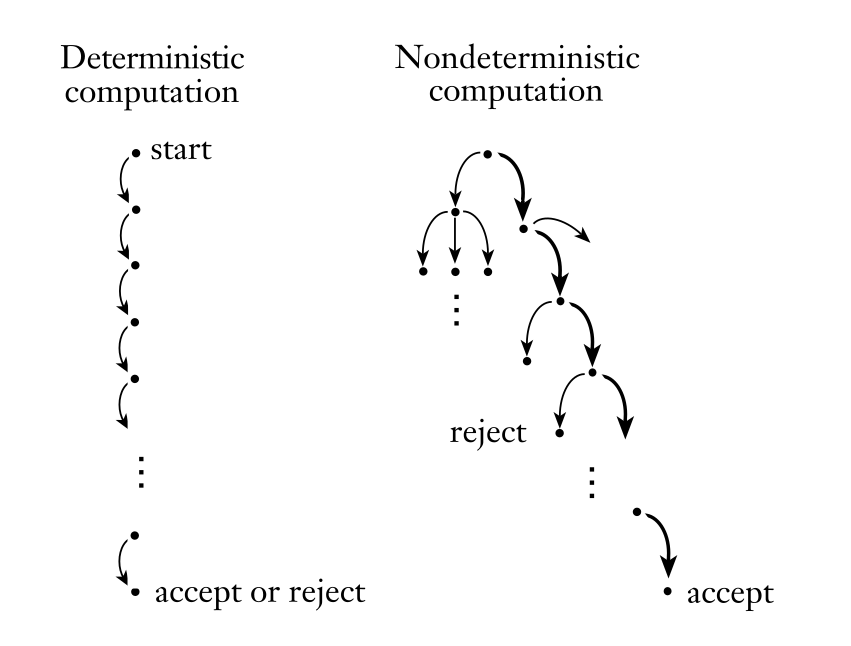
\includegraphics[width=\textwidth]{figur/figure128.png}
	\end{figure}

\end{frame}

\begin{frame}[allowframebreaks]
	\frametitle{Formel NFA}

	En \textit{nondeterministik endelig automat} er en 5-tuple ($Q, \Sigma, \delta, q_{0}, F$), hvor:

	\begin{enumerate}
		\item $Q$ er en endelig mængde af tilstande
		\item $\Sigma$ er et endeligt alfabet
		\item $\delta : \Sigma_{\varepsilon} \longrightarrow \mathcal{P}(Q)$ er overføringsfunktionen
		\item $q_{0} \in Q$ er start tilstanden
		\item $F \subseteq Q$ er mængden af accept tilstande
	\end{enumerate}

	Her er $\mathcal{P}(Q)$ ``power set'' af $Q$, altså alle kombinationer af tilstandende, inklusiv den tomme mængde.
\end{frame}

\begin{frame}[allowframebreaks]
	\frametitle{NFA ækvivalens med DFA}
	\begin{itemize}
		\item Som sagt før er en NFA i samme sprogklasse som en DFA. Dette kalder vi at de er \textit{ækvivalente.} Dette vil altså betyde at en NFA kan genkende sprog $A \iff $ en DFA kan genkende sprog $A$.
		\item Den ækvivalente DFA (dvs. en DFA der genkender samme sprog som en specifik NFA) vil have $2^{k}$ tilstande, hvor $k$ er antallet af tilstande i NFA'en. Vi vil nu bevise ved konstruktion:
		\item Lad $N = (Q, \Sigma, \delta, q_{0}, F)$ være en NFA der genkender et sprog, $A$. Lad $M = (Q', \Sigma, \delta', q_{0}', F')$ være en DFA der genkender $A$. Vi antager først at $N$ ikke har nogen epsilon-pile, og kigger i stedet på dette efter konstruktionen.
		      \begin{enumerate}
			      \item $Q' = \mathcal{P}(Q)$. \\ Hver tilstand i $M$ er en mængde af tilstande i $N$.
			      \item For $R \in Q'$ og $a \in \Sigma$, lad $\delta'(R,a) = \{q \in Q \mid q \in \delta(r,a) \text{ for en } r \in R\}$. En anden måde at skrive dette på er:
			            \begin{equation*}
				            \delta'(R,a) = \bigcup_{r \in R} \delta(r,a)
			            \end{equation*}
			      \item $q_{0}' = \{q_{0}\}$
			      \item $F' = \{R \in Q' \mid R \text{ indeholder en accept tilstand af }N\}$  \\ Hvis en af tilstandene er en accepterende tilstand, er mængden indeholdende en af disse tilstande, også accepterende.
		      \end{enumerate}
		\item Hvis vi tilføjer epsilon-pile, skal vi bruge lidt mere til overførselsfunktionen.
		\item Først definerer vi $E(R)$ til at være samllingen af tilstande som kan nås fra medlemmer af $R$ kun ved at gå langs $\varepsilon$-pile, inklusiv medlemmer i $R$ selv. For $R \subseteq Q$ lad: \begin{equation*}
			      E(R) = \{q \mid q \text{ kan nås fra } R \text{ ved at gå langs 0 eller flere } \varepsilon \text{ pile.}\}
		      \end{equation*}
		\item Vi ændrer nu overførselsfunktionen således: \begin{equation*}
			      \delta' (R,a) = \{q \in Q \mid q \in E(\delta(r,a)) \text{ for en } r \in R\}
		      \end{equation*}
		\item Derudover skal vi også ændre $q_{0}$, da det nu er muligt at effektivt have mere end én starttilstand. Dermed $q_{0} = E(\{q_{0}\})$.
	\end{itemize}
\end{frame}

\begin{frame}[allowframebreaks]
	\frametitle{Regulære Sprog er lukket under fællesmængde}
	\begin{itemize}
		\item Vi har allerede bevist dette ved hjælp af DFA'er, men nu kigger vi på et langt mere intuitivt bevis med NFA'er. Desuden bruger vi kun visuelle midler:
	\end{itemize}
	\begin{figure}
		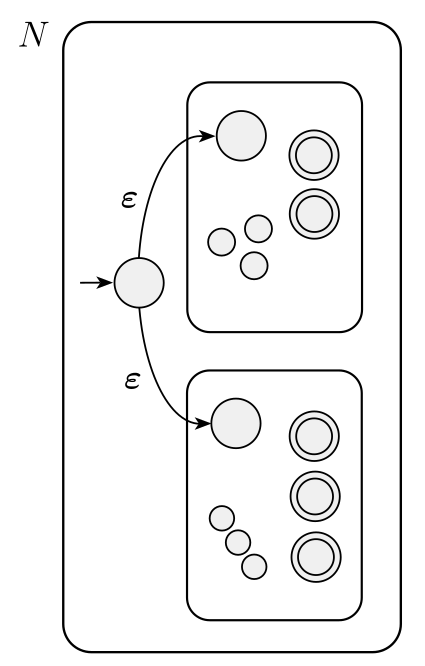
\includegraphics[scale=0.5]{figur/figur146.png}
	\end{figure}
\end{frame}

\begin{frame}[allowframebreaks]
	\frametitle{Regulære Sprog er lukket under sammenkædning}

	\begin{itemize}
		\item Igen bruger vi NFA til at bevise.
		\item I sin essens: Vi har to endelige automater $M_{1}$ og $M_{2}$. For at få $M_{1} \circ M_{2}$ tager vi mængden $F$ i $M_{1}$ og konverterer til almindelige tilstande (altså fjerner deres accept).
		\item De tilstande der nu er almindelige, men før var accepterende, går \textbf{alle} til starttilstanden af $M_{2}$.
	\end{itemize}

	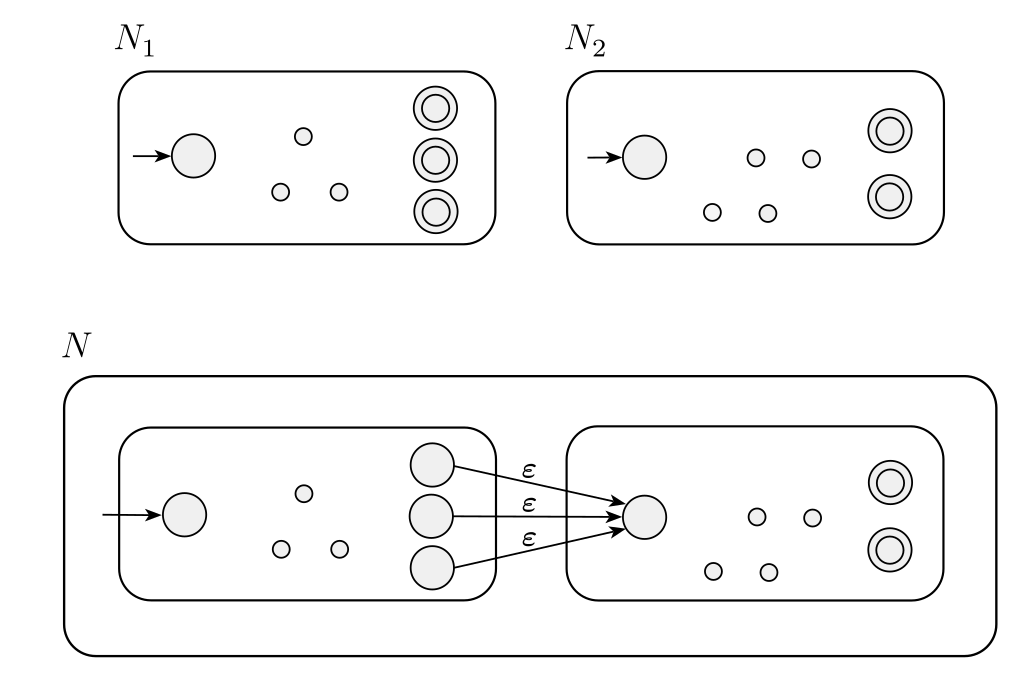
\includegraphics[width=\textwidth]{figur/figur148.png}
\end{frame}

\begin{frame}[allowframebreaks]
	\frametitle{Regulære Sprog er lukket under stjerne}

	\begin{itemize}
		\item Visuelt bevis:
	\end{itemize}
	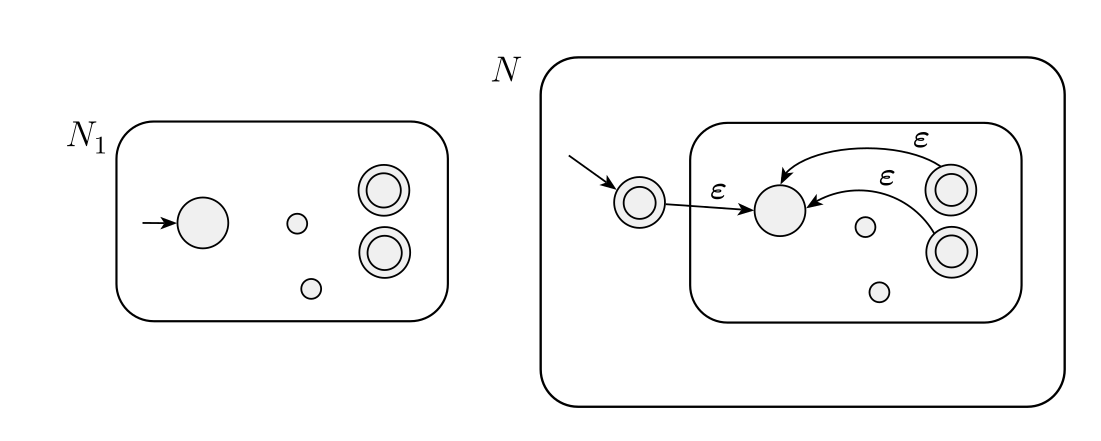
\includegraphics[scale=0.4]{figur/figur150.png}
\end{frame}

\subsection{Regulære Udtryk}%
\label{subsec:regulæreudtryk}

\begin{frame}
	\frametitle{Regulære Udtryk}
	\begin{itemize}
		\item Regulære udtryk er udtryk for et regulært sprog.
		\item For eksempel er det regulære udtryk $(0 \cup 1)0^{*}$ et udtryk for sproget af alle strenge der starter med et 0 eller et 1, efterfulgt af 0 eller flere 0'er.
		\item Ligesom $\times$ i algebra, er $\circ$ (sammenkædning) ofte implicit mellem symboler.
	\end{itemize}
\end{frame}

\begin{frame}[allowframebreaks]
	\frametitle{Formel definition af regulære udtryk}
	\begin{itemize}
		\item $R$ er et \textit{regulært udtryk} hvis $R$ er:
		      \begin{enumerate}
			      \item $a$ for en $a$ i $\Sigma$
			      \item $\varepsilon$
			      \item $\emptyset$
			      \item $(R_{1} \cup R_{2})$, hvor $R_{1}$ og $R_{2}$ er regulære udtryk
			      \item $(R_{1} \circ R_{2})$, hvor $R_{1}$ og $R_{2}$ er regulære udtryk
			      \item $(R_{1}^{*})$ hvor $R_{1}$ er et regulært udtryk.
		      \end{enumerate}
		\item Her betyder 1. og 2. hhv. sprogene $\{a\}$ og $\{\varepsilon\}$.
	\end{itemize}
\end{frame}

\begin{frame}[allowframebreaks]
	\frametitle{Ækvivalens med endelige automater}
	\begin{itemize}
		\item Et sprog er regulært $\iff$ et regulært udtryk genkender det.
		\item Jeg vil ikke vise at \textit{hvis et regulært udtryk genkender et sprog, er det regulært}, da det bare er at konvertere hver ting til dele af en endelig automat.
		\item Den anden side, altså \textit{Et sprog er regulært \(\Rightarrow\) et regulært udtryk genkender det} bruger vi \textit{GNFA} til.
		\item En GNFA er blot en generaliseret nondeterministisk endelig automat.
		\item Denne tillader regulære udtryk.
		\item Vores mål er at reducere to pile til et udtryk, og dermed ende med to tilstande, en start og en slut, hvorpå det regulære udtryk udfolder sig.
	\end{itemize}
\end{frame}

\subsection{Non-regulære sprog}%
\label{subsec:nonregulæresprog}

\begin{frame}
	\frametitle{Non-regulære sprog}
	\begin{itemize}
		\item Som vi forhåbentligt allerede ved, genkender endelige automater ikke \textit{alle} mulige sprog.
		\item Sprog der ikke er en del af klassen af regulære sprog, kaldes \textit{non-regulære sprog}.
		\item Et eksempel på et sådan sprog er sproget $B = \{0^{n}1^{n} \mid n \ge 0\}$
		\item Det er relativt nemt at se at dette sprog ikke er regulært, da det kræver potentielt uendelig hukommelse, og en \textit{endelig} automat har endelig hukommelse.
		\item Bemærk dog at dette \textbf{ikke} betyder at alle uendelige sprog ikke er regulære. Følgende er et eksempel på et sprog der er uendeligt \textit{og} regulært:
		\item $D = \{w \mid w \text{ har et lige antal af forekomster af \texttt{01} og \texttt{10} som delstrenge}\}$
		\item Dermed skal vi have matematiske beviser for hvorfor noget \textit{ikke} er regulært.
	\end{itemize}
\end{frame}

\begin{frame}[allowframebreaks]
	\frametitle{Pumpelemmaet}
	\begin{itemize}
		\item Pumpelemmaet siger at alle regulære sprog har en speciel egenskab. Hvis vi kan bevise mangel på denne, beviser vi dermed også at vi har at gøre med et non-regulært sprog.
		\item Denne egenskab er at alle strenge af en minimumslængde kan blive ``pumpet'' i sproget.
		\item Altså kan der findes en del af hver streng som kan blive pumpet et arbitrært antal gange, hvor det forbliver i sproget.
	\end{itemize}

	\begin{theorem}[Pumpelemmaet]
		Hvis $A$ er et endeligt sprog, så eksisterer der et tal $p$ (pumpelængden), hvor, hvis $s$ er en streng i $A$ af længde mindst $p$, så kan $s$ deles i tre stykker, således at $s = xyz$, og $s$ overholder følgende betingelser:
		\begin{enumerate}
			\item For hvert $i \ge 0$, $xy^{i}z \in A$ \\ Altså skal strengen altid kunne deles op således at $y$-delen kan pumpes uendeligt mange gange, og blive i strengen.
			\item $|y| > 0$ \\ Hvis $y = \varepsilon$ (som denne betingelse ikke tillader), er dette altid sandt da $\varepsilon^{i}$ hvor $i \ge 0$  giver $\varepsilon$, som naturligvis stadig er i sproget.
			\item $|xy| \le p$
		\end{enumerate}
	\end{theorem}
\end{frame}

\begin{frame}[allowframebreaks]
	\frametitle{Bevis på Pumpelemmaet}
	\begin{itemize}
		\item Lad os nu bevise at pumpelemmaet er sandt.
	  \item Givet en DFA $A$, og en pumpelængde $p$\footnote{Vi angiver $p$ til at være antallet af tilstande i $A$}, vil vi gerne vise at enhver streng $v$ hvor $|v| \ge p$ kan splittes til tre delstrenge $xyz = v$.
	  \item Hvis $\{\forall v \in L(A)  \mid |v| \ge p\} = \emptyset$ er sætningen sand for $A$.
	  \item For enhver anden streng der overholder $|v| \ge p$, kan vi se på denne strengs gennemgang af $A$ som en sekvens: $q_{1}, q_{9}, q_{4}, \ldots, q_{10}$\footnote{Eksempel tilstande, ikke en reel gennemgang} hvor $q_{1}$ er starttilstanden og $q_{10}$ er accepttilstanden.
	  \item Da vi ved at $|v| \ge p$ og $p = |Q|$, og for hver karakter i $v$ går vi igennem en tilstand plus starttilstanden, må antallet af tilstande i gennemgangen være $|v| + 1$.
	  \item Dermed gælder det at $|v| + 1 > |Q|$.
	  \item Dette betyder at der \textbf{må} være en tilstand som er gentagen.\footnote{Fra dueslagsprincippet.}
	  \item Da vi kan sikre at der er mindst én gentagen tilstand, kan vi splitte strengen op således at $x$ er strengen før den gentagne tilstand. $y$ er fra den første gentagende tilstand til den bliver gentaget. $z$ er resterende.
	  \item Vi vil nu vise at denne opdeling af $s$ opfylder betingelserne:
			\begin{enumerate}
			  \item $y$ kan gentages så mange gange vi vil, inklusiv $0$
			  \item $y > 0$ er sikret, da den gentagne del af gennemgangen skal være $y \ge 1$ (1 hvis e.g. $q_{0}, q_{0}$)
			  \item For at sikre $|xy| \le p$ skal $y$ starte ved den første gentagne tilstand. Fra dueslagsprincippet må gentagningen ske indenfor de først $p+1$ tilstande.
 			\end{enumerate}
	  \item For at bruge pumpelemmaet til at bevise nonregulæritet af et sprog $B$, antager vi først at sproget $B$ er regulært for at kunne finde et modstrid.
	\end{itemize}
\end{frame}

\begin{frame}
  \frametitle{Eksempel 1.75}

  \begin{itemize}
	\item Vi kigger hurtigt på et eksempel:
	\item Lad $F = \{ww \mid w \in \{\text{\texttt{0,1}}\}^{*}\}$
	\item Vi bruger strengen $0^{p}10^{p}1$
	\item Grundet betingelse 3 $|xy| \le p$ er det umuligt at pumpe denne, da $xy = 00 \ldots 00$ da vi ved at der er $p$ \texttt{0}'er.
	\item Bemærk her at vi \textit{ikke} kunne bruge f.eks. strengen $0^{p}0^{p}$, da den ville være i $F$.
	\item Dermed kræver det også lidt kreativitet.
  \end{itemize}
\end{frame}

\begin{frame}
  \frametitle{Eksempel 1.76}
 \begin{itemize}
   \item Givet $D = \{1^{n^{2}}\}$
   \item Vi vælger strengen $1^{p^{2}}$
   \item Fra betingelse 3: $|xy| \le p$
   \item Dermed $|y| \le p$
   \item Dermed $|xyz| \le p^{2}$ og $|xy^{2}z| \le p^{2}+p$, hvor vi ønsker $(p+1)^{2} = p^{2} + 2p + 1$
 \end{itemize}
\end{frame}


\begin{frame}
  \frametitle{Eksempel 1.77}
 \begin{itemize}
   \item<1-> Sidste eksempel: nedpumpning
   \item<1-> Givet $E = \{0^{i}1^{j} \mid i > j\}$
   \item<1-> $s = 0^{p+1}1^{p}$
   \item<1-> Det virker umuligt at, for $0^{p+1}1^{p}$, uanset pumpingen vil \texttt{0} vel stadig være større? Hvad gør vi?
   \item<2> Som hintet: vi nedpumper! $y^{0} = \varepsilon$, og da $|y| \ge 1$ er $i$ enten mindre end eller lig med $j$.
 \end{itemize}
\end{frame}


\subsection{Non-kontekstfrie sprog}%
\label{subsec:nonkontekstfriesprog}

\begin{frame}
  \frametitle{Non-kontekstfrie sprog}
  \begin{itemize}
	\item Ligesom ved regulære sprog, er der nogle sprog der \textbf{ikke} er kontekstfrie. Husk at $RL \subset CFL$\footnote{RL = Regular Languages, CFL = Context-Free Languages}, og dermed hvis et sprog ikke er regulært er det heller ikke kontekstfrit.
  \end{itemize}
\end{frame}

\begin{frame}[allowframebreaks]
  \frametitle{Pumpelemmaet for kontekstfrie sprog}

  \begin{theorem}[Pumpelemma for kontekstfrie sprog]
	Hvis $A$ er et kontekstfrit sprog, så er der et tal $p$ (pumpelængden) hvor, hvis $s$ er i nogen strenge i $A$ af længde mindst $p$, så kan $s$ opdelees til fem stykker $s = uvxyz$ som opfylder de følgende betingelser:
	\begin{itemize}
	  \item For hvert $i \ge 0$, $uv^{i}xy^{i}z \in A$
	  \item $|vy| > 0$
	  \item $|vxy| \le p$
	\end{itemize}
  \end{theorem}
  \begin{itemize}
	\item Her siger betingelse 2 at \textit{enten} $v$ eller $y$ ikke er den tomme streng.
	\item Betingelse 3 siger at delene $v, x$ og $y$ sammen har længde højest $p$.
  \end{itemize}
  \item Lad os nu bevise.
\end{frame}


%%% Local Variables:
%%% mode: latex
%%% TeX-engine: xetex
%%% TeX-command-extra-options: "-shell-escape"
%%% TeX-master: "main"
%%% End:
